\documentclass[11pt]{article}
\pagestyle{empty}
\setlength{\parindent}{0pt}
\usepackage[simplified]{pgf-umlcd}
\usepackage{tikz}
\usepackage[margin=0.5cm]{geometry}  % Set narrow page margins

\begin{document}
    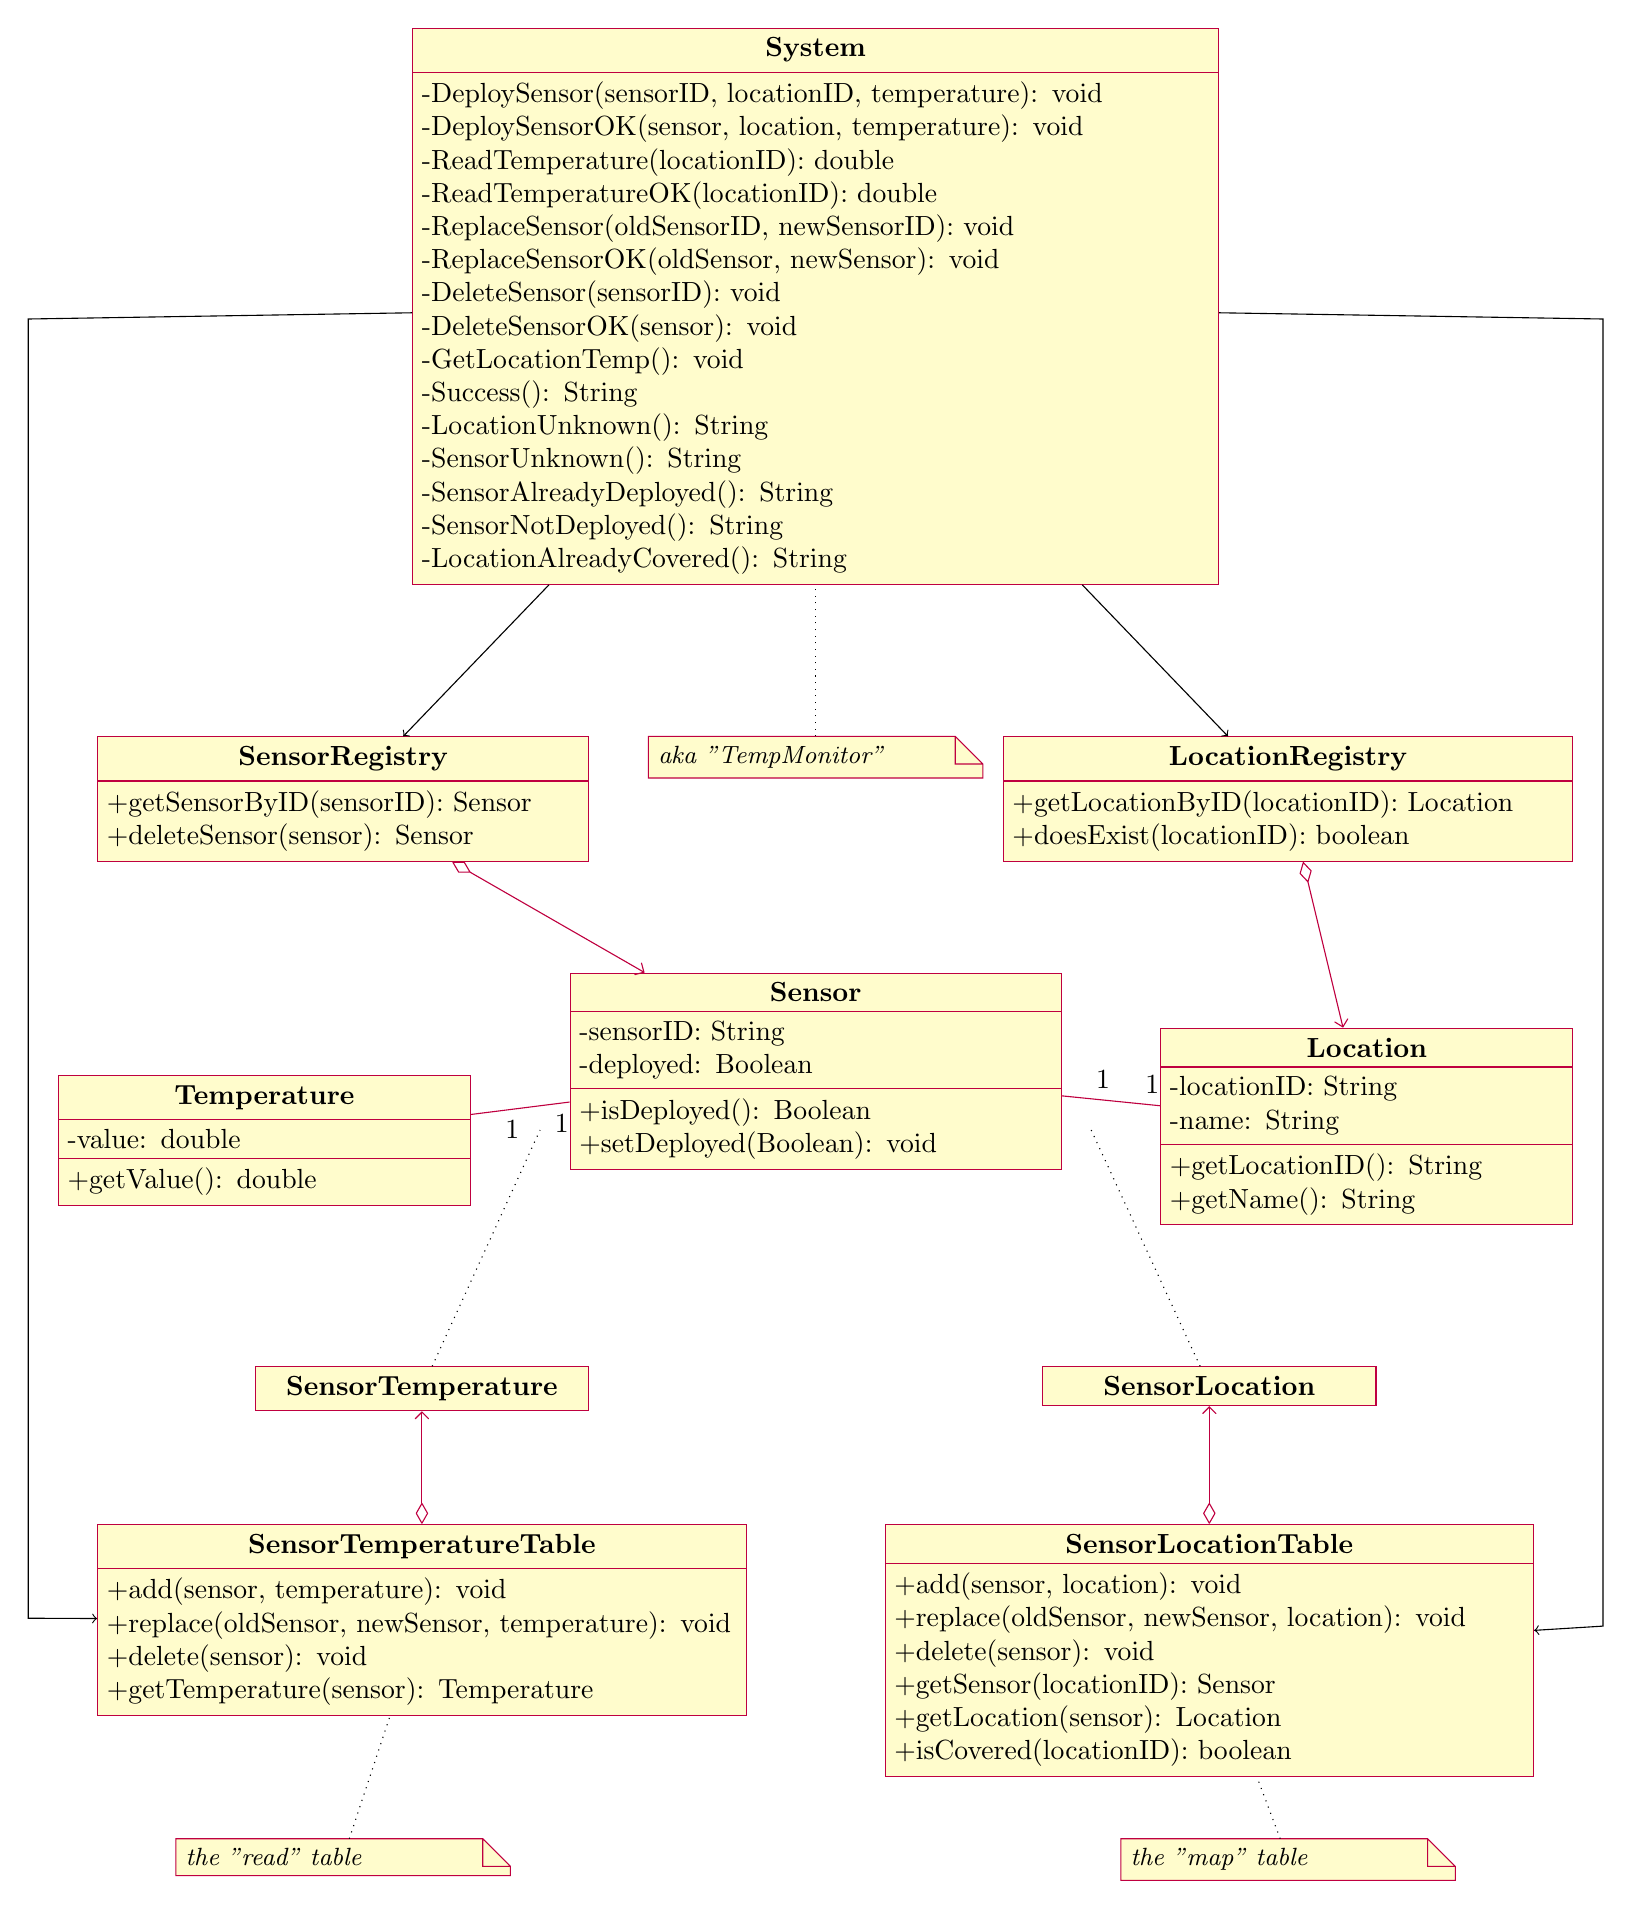
\begin{tikzpicture}
        % Defining the classes and their attributes
        \begin{class}[text width=10cm]{System}{2, 8}
            \operation{-DeploySensor(sensorID, locationID, temperature): void}
            \operation{-DeploySensorOK(sensor, location, temperature): void}
            \operation{-ReadTemperature(locationID): double}
            \operation{-ReadTemperatureOK(locationID): double}
            \operation{-ReplaceSensor(oldSensorID, newSensorID): void}
            \operation{-ReplaceSensorOK(oldSensor, newSensor): void}
            \operation{-DeleteSensor(sensorID): void}
            \operation{-DeleteSensorOK(sensor): void}
            \operation{-GetLocationTemp(): void}
            \operation{-Success(): String}
            \operation{-LocationUnknown(): String}
            \operation{-SensorUnknown(): String}
            \operation{-SensorAlreadyDeployed(): String}
            \operation{-SensorNotDeployed(): String}
            \operation{-LocationAlreadyCovered(): String}
        \end{class}
        
        \begin{class}[text width=6cm]{SensorRegistry}{-4,-1}
            \operation{+getSensorByID(sensorID): Sensor}
            \operation{+deleteSensor(sensor): Sensor}
        \end{class}
        
        \begin{class}[text width=6cm]{Sensor}{2,-4}
            \attribute{-sensorID: String}
            \attribute{-deployed: Boolean}
            \operation{+isDeployed(): Boolean}
            \operation{+setDeployed(Boolean): void}
            
        \end{class}
        
        \begin{class}[text width=7cm]{LocationRegistry}{8,-1}
            \operation{+getLocationByID(locationID): Location}
            \operation{+doesExist(locationID): boolean}
        \end{class}

        \begin{class}[text width=5cm]{Location}{9,-4.7}
            \attribute{-locationID: String}
            \attribute{-name: String}
            \operation{+getLocationID(): String}
            \operation{+getName(): String}
        \end{class}

        \begin{class}[text width=5cm]{Temperature}{-5,-5.3}
            \attribute{-value: double}
            \operation{+getValue(): double}
        \end{class}

        \begin{class}[text width=4cm]{SensorTemperature}{-3,-9}
        \end{class}

        \begin{class}[text width=4cm]{SensorLocation}{7,-9}
        \end{class}

        \begin{class}[text width=8cm]{SensorTemperatureTable}{-3,-11}
            \operation{+add(sensor, temperature): void}
            \operation{+replace(oldSensor, newSensor, temperature): void}
            \operation{+delete(sensor): void}
            \operation{+getTemperature(sensor): Temperature}
        \end{class}

        \begin{class}[text width=8cm]{SensorLocationTable}{7,-11}
            \operation{+add(sensor, location): void}
            \operation{+replace(oldSensor, newSensor, location): void}
            \operation{+delete(sensor): void}
            \operation{+getSensor(locationID): Sensor}
            \operation{+getLocation(sensor): Location}
            \operation{+isCovered(locationID): boolean}
        \end{class}

        % Defining the links between the classes
        \association {Sensor}{1}{}{Location}{1}{}
        \association {Sensor}{1}{}{Temperature}{1}{}
        \aggregation{SensorRegistry}{}{}{Sensor}
        \aggregation{LocationRegistry}{}{}{Location}
        \aggregation{SensorLocationTable}{}{}{SensorLocation}
        \aggregation{SensorTemperatureTable}{}{}{SensorTemperature}

        % Manual associations
        \draw[->] (System) -- (SensorRegistry);
        \draw[->] (System) -- (LocationRegistry);
        \draw[->] (System) -- (12, 4.3) -- (12, -12.3) -- (SensorLocationTable);
        \draw[->] (System) -- (-8, 4.3) -- (-8, -12.2) -- (SensorTemperatureTable);
        \draw[dotted] (SensorTemperature) -- (-1.5, -6);
        \draw[dotted] (SensorLocation) -- (5.5, -6);

        % Notes
        \umlnote(note1) at (2,-1){\textit{\small aka "TempMonitor"}};
        \draw[dotted] (note1) -- (System);
        \umlnote(note2) at (-4,-15){\textit{\small the "read" table}};
        \draw[dotted] (note2) -- (SensorTemperatureTable);
        \umlnote(note3) at (8,-15){\textit{\small the "map" table}};
        \draw[dotted] (note3) -- (SensorLocationTable);
    
    \end{tikzpicture}
\end{document}
